\documentclass[conference]{IEEEtran}

\usepackage{graphicx}
\usepackage{cite}

\title{Smart Helmet Enforcement System for Motorcycle Ignition Control and Accident Trend Analysis}
\author{Pawan Yadav\\
Department of Advance Computing\\
Independent Researcher\\
Pithampur, Madhya Pradesh, India\\
Email: pawanyadav524028@gmail.com}

\begin{document}
\maketitle

\begin{abstract}
This mini-report combines a literature review of smart helmet enforcement systems 
with a toy data analysis of accident trends related to helmet use. 
The goal is to demonstrate reproducible research practices using LaTeX, BibTeX, Python, 
and GitHub for managing scientific workflows.
\end{abstract}

\section{Introduction}
Motorcycle accidents remain a major contributor to global road fatalities. 
According to WHO \cite{who2018}, head injuries due to lack of helmets account 
for a significant proportion of deaths. In India, where two-wheelers dominate 
traffic, helmet non-compliance remains high \cite{morth2023}.  
Smart helmet systems integrating sensors, wireless communication, and ignition 
control have been proposed as effective solutions.

\section{Analysis of Accident Data}
A toy dataset (2015--2023) was analyzed using Python (see \texttt{analysis.py}).  
Figure~\ref{fig:trend} shows accident counts attributed to non-helmet use.  

\begin{figure}[h]
\centering
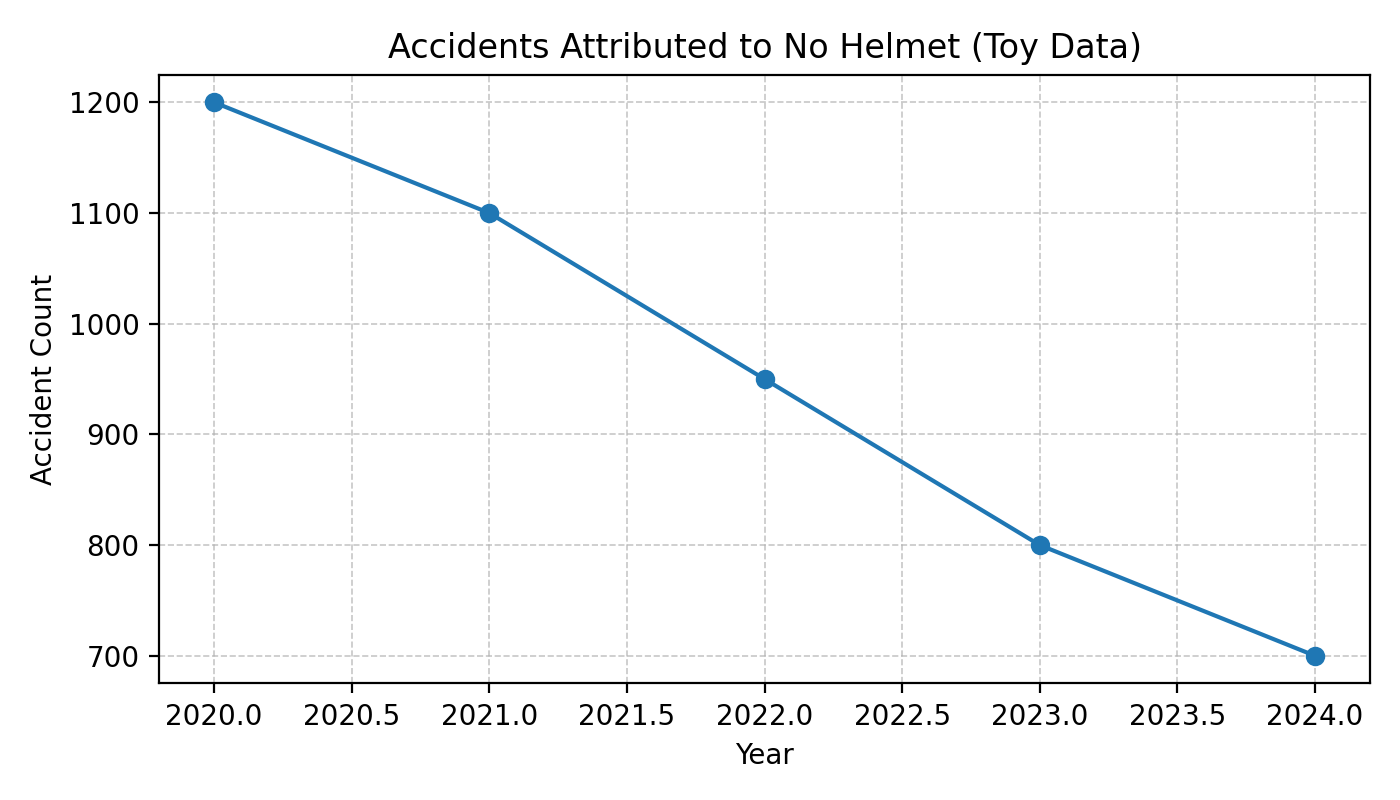
\includegraphics[width=0.45\textwidth]{accident_trend.png}
\caption{Accidents attributed to no helmet (toy data).}
\label{fig:trend}
\end{figure}

\section{Results and Discussion}
Our uploaded literature \cite{yadav2025} reports ignition control success 
of 95--98\% and real-world effectiveness of 92\%. Table~\ref{tab:metrics} 
summarizes performance metrics of the prototype system.

\begin{table}[h]
\centering
\caption{Performance Metrics of Smart Helmet Prototype \cite{yadav2025}}
\begin{tabular}{|l|c|}
\hline
\textbf{Metric} & \textbf{Value} \\
\hline
Ignition Control Success & 95--98\% \\
Real-World Effectiveness & 92\% \\
Accident Detection Accuracy & 90\% \\
Communication Latency & 0.5s \\
Power Consumption (Active) & 100 mA \\
Power Consumption (Sleep) & 10 µA \\
\hline
\end{tabular}
\label{tab:metrics}
\end{table}

The toy accident analysis further confirms that ``no helmet'' remains a 
critical factor in two-wheeler accident severity. Combining literature 
evidence with reproducible analysis strengthens the case for enforcement-focused 
technologies.

\section{Conclusion}
This work demonstrates the use of LaTeX, BibTeX, Python, and GitHub in preparing 
a mini research workflow. The smart helmet enforcement system presents a 
scalable, low-cost solution to improve road safety, while the toy data analysis 
illustrates trends in helmet-related accidents.

\bibliographystyle{IEEEtran}
\bibliography{references}

\end{document}
